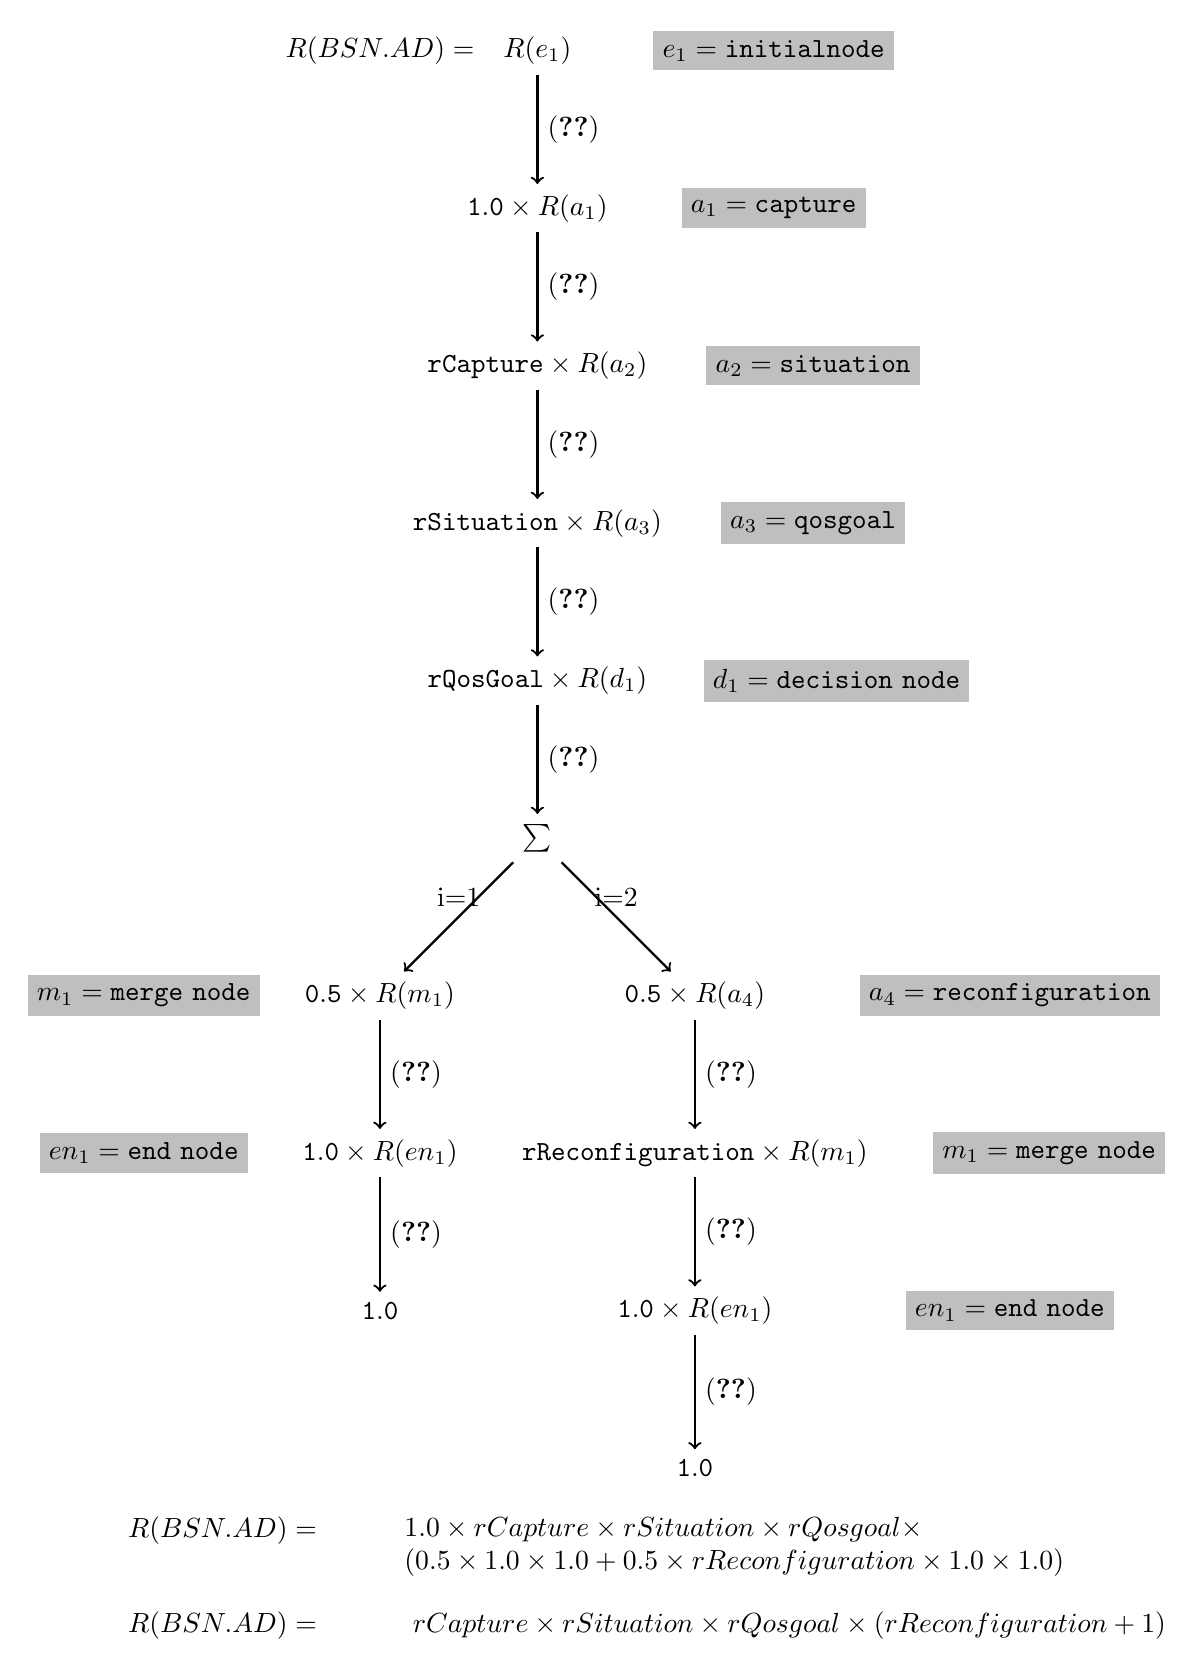
\begin{tikzpicture}[thick]
% \draw[help lines, step=1cm] (0,0) grid +(10,20); 
%%%%%%%%%%%%%%%%%%%%%%%%%%%%%%% Derivation tree for BSN AD
\node[rectangle, draw=none](rBsnAd) at (3.0,20){$R(BSN.AD)=$};
\node[rectangle, draw=none](rinit) at (5,20){$R(e_1)$};
\node[rectangle, draw=none, fill=gray!50](obsBsnAd) at(8,20){$e_1 = \mathtt{initial node}$};
% \draw[->,thick] (rinit) -- node[draw=none,auto]{()}();

\node[rectangle, draw=none](rA1) at (5,18){$\mathtt{1.0} \times R(a_1)$};
\node[rectangle, draw=none, fill=gray!50](obsA1) at(8,18){$a_1 = \mathtt{capture}$};
\draw[->,thick] (rinit) -- node[draw=none,auto]{(\ref{eq:initialNodeReliability})}(rA1);

\node[rectangle, draw=none](rA2) at (5,16){$\mathtt{rCapture} \times R(a_2)$};
\node[rectangle, draw=none, fill=gray!50](obsA2) at(8.5,16){$a_2 = \mathtt{situation}$};
\draw[->,thick] (rA1) -- node[draw=none,auto]{(\ref{eq:activityReliability})}(rA2);

\node[rectangle, draw=none](rA3) at (5,14){$\mathtt{rSituation} \times R(a_3)$};
\node[rectangle, draw=none, fill=gray!50](obsA3) at(8.5,14){$a_3 = \mathtt{qosgoal}$};
\draw[->,thick] (rA2) -- node[draw=none,auto]{(\ref{eq:activityReliability})}(rA3);

\node[rectangle, draw=none](rD1) at (5,12){$\mathtt{rQosGoal} \times R(d_1)$};
\node[rectangle, draw=none, fill=gray!50](obsD1) at(8.8,12){$d_1 = \mathtt{decision\ node}$};
\draw[->,thick] (rA3) -- node[draw=none,auto]{(\ref{eq:activityReliability})}(rD1);

\node[rectangle, draw=none](rSum) at (5,10){$\sum$};
\draw[->,thick] (rD1) -- node[draw=none,auto]{(\ref{eq:decisionNodeReliability})}(rSum);
% \draw[->,thick] () -- node[draw=none,auto]{()}();

\node[rectangle, draw=none](rM1) at (3,8){$\mathtt{0.5} \times R(m_1)$};
\node[rectangle, draw=none, fill=gray!50](obsM1) at(0,8){$m_1 = \mathtt{merge\ node}$};
\draw[->,thick] (rSum) -- node[draw=none,above]{i=1}(rM1);

\node[rectangle, draw=none](rE1) at (3,6){$\mathtt{1.0} \times R(en_1)$};
\node[rectangle, draw=none, fill=gray!50](obsBsnAd) at(0,6){$en_1 = \mathtt{end\ node}$};
\draw[->,thick] (rM1) -- node[draw=none,auto]{(\ref{eq:mergeNodeReliability})}(rE1);

\node[rectangle, draw=none](ren1) at (3,4){$\mathtt{1.0}$};
\draw[->,thick] (rE1) -- node[draw=none,auto]{(\ref{eq:endNodeReliability})}(ren1);

\node[rectangle, draw=none](rA4) at (7,8){$\mathtt{0.5} \times R(a_4)$};
\node[rectangle, draw=none, fill=gray!50](obsA4) at(11,8){$a_4 = \mathtt{reconfiguration}$};
\draw[->,thick] (rSum) -- node[draw=none,above]{i=2}(rA4);

\node[rectangle, draw=none](rM1) at (7,6){$\mathtt{rReconfiguration} \times R(m_1)$};
\node[rectangle, draw=none, fill=gray!50](obsM1) at(11.5,6){$m_1 = \mathtt{merge\ node}$};
\draw[->,thick] (rA4) -- node[draw=none,auto]{(\ref{eq:activityReliability})}(rM1);

\node[rectangle, draw=none](ren1) at (7,4){$\mathtt{1.0} \times R(en_1)$};
\node[rectangle, draw=none, fill=gray!50](obsEn1) at(11,4){$en_1 = \mathtt{end\ node}$};
\draw[->,thick] (rM1) -- node[draw=none,auto]{(\ref{eq:mergeNodeReliability})}(ren1);

\node[rectangle, draw=none](rTerm) at (7,2){$\mathtt{1.0}$};
\draw[->,thick] (ren1) -- node[draw=none,auto]{(\ref{eq:endNodeReliability})}(rTerm);

\node[rectangle, draw=none](rBsnAd) at (1.0,1.2){$R(BSN.AD)= $};
\node[rectangle, draw=none,align=left](rBsnAd) at (7.5,1){$1.0 \times rCapture \times rSituation \times rQosgoal \times $\\$(0.5 \times 1.0 \times 1.0 + 0.5 \times rReconfiguration \times 1.0 \times 1.0) $};
\node[rectangle, draw=none](rBsnAd) at (1.0,0){$R(BSN.AD)= $};
\node[rectangle, draw=none,align=left](rBsnAd) at (8.2,0){$rCapture \times rSituation \times rQosgoal \times ( rReconfiguration + 1) $};

\end{tikzpicture}

